\documentclass[11pt]{article}
\usepackage{geometry}                % See geometry.pdf to learn the layout options. There are lots.
\usepackage{graphicx}
\usepackage{amssymb}
\usepackage{epstopdf}
\usepackage{algorithmic}
\usepackage{algorithm}
\usepackage{url}
\usepackage{framed}
\usepackage{amssymb}
\usepackage{amsmath}
 

\title{Homework 1}                                   % Activate to display a given date or no date

\begin{document}
\maketitle

\section*{\textbf{Due: September 13, 2018, 11:59 PM EST}}

\section*{\textbf{Instructions}}

Your homework submission must cite any references used (including articles, books, code, websites, and personal communications). All solutions must be written in your own words, and you must program the algorithms yourself. If you do work with others, you must list the people you worked with. If you solve any problems by hand just digitize that page and submit it (make sure the problem is labeled). \\

\noindent Your programs must be written in Python.  All code \underline{must} be able to compile and run for full credit.  Comment all code following proper coding conventions. Remember, if we can't read it, we can't grade it! (For more information on python coding standards, refer to: \emph{https://www.python.org/dev/peps/pep-0008/}) \\

\noindent You should submit your assignment via Github.  Submit your solutions as a PDF named ''hw(hw \#).pdf''.  For example, homework 1 should be submitted as hw01.pdf.  If the assignment requires coding, submit your \underline{working} code as a .py file with the same name. \\



If you have any questions address them to:
\begin{itemize}
\item Connor McCurley (TA) -- cmccurley@ufl.edu
\item Xiaolei Guo (TA) -- suninth@ufl.edu
\item Daniel Wells (TA) -- dwells@ufl.edu
\end{itemize}

\pagebreak

\section*{Question 1 - 3.5 points}
Consider the polynomial curve fitting example discussed in class. As discussed, when the model order is \emph{too} small, the training data is generally \emph{underfit} and when the model order is \emph{too} high, the result can \emph{overfit} the training data.  Write a small script of code that mimics our polynomial curve fitting function.  The code should generate simulated data from the true function with added zero-mean Gaussian noise (with the true function assumed to be sinc function). The code should also generate a separate validation test data set generated in the same way.  Then, after fitting the polynomial to the training data across a range of model orders and evaluated on both the training and testing data, your code should generate a plot similar to the one shown in Figure 1.  Also, provide a discussion based on your plot about which model order, $M$, should be used to avoid over-training.

\[  sinc(x) = \left\{
\begin{array}{ll}
      1 & for \: x=0 \\
      \frac{sin(x)}{x} & otherwise\\
\end{array} 
\right. \]

\begin{figure}[h!]
\centering
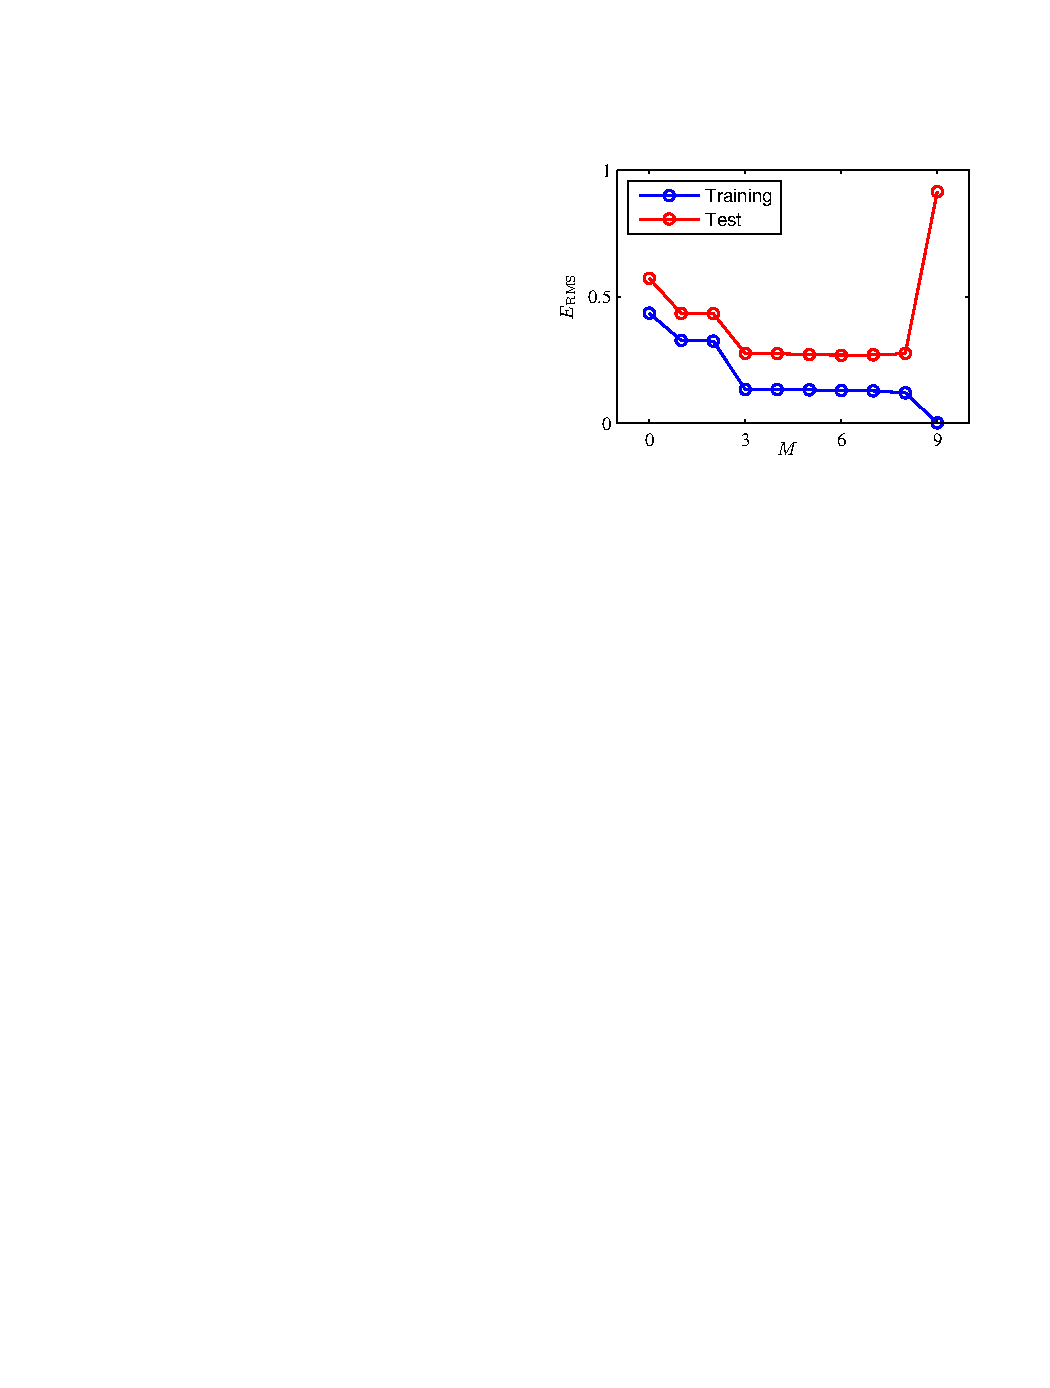
\includegraphics{problem1.pdf}
\caption{Figure 1.5 from the Bishop textbook.  The y-axis corresponds to the root-mean-square error between the predicted and the true value (on either the training data or test data sets).  The x-axis corresponds to the model order. }
\end{figure}

\section*{Question 2 - 4.5 points}

\subsection*{Recall:}

Assuming a univariate Gaussian data likelihood given $N$ i.i.d. data points:

\begin{equation}
p(\mathbf{X}|\mu) = \prod^{N}_{n=1}\mathcal{N}(x_n|\mu,\sigma^2)
\end{equation}

and a Gaussian prior distribution on the mean:

\begin{equation}
p(\mu|\mu_0) = \mathcal{N}(\mu|\mu_0,\sigma^{2}_{0})
\end{equation}

with fixed variances ($\sigma^2, \sigma^{2}_{0}$, and $\sigma^2 \neq \sigma^{2}_{0}$), the posterior distribution is given by:

\begin{equation}
p(\mu|\mathbf{X}) = \mathcal{N}(\mu|\mu_N,\sigma^{2}_{N})
\end{equation}

where

\begin{equation}
\mu_N = \frac{\sigma^2}{N\sigma^{2}_{0} + \sigma^2}\mu_0 + \frac{N\sigma^{2}_{0}}{N\sigma^{2}_{0} + \sigma^2}\mu_{ML}
\end{equation}

\begin{equation}
\frac{1}{\sigma^{2}_{N}} = \frac{1}{\sigma^{2}_0} + \frac{N}{\sigma^{2}}
\end{equation}

where $\mu_{ML}$ is the maximum likelihood solution for $\mu$ given the $N$ data points.

\begin{itemize}
	\item In or Binomial/Beta example in class, we computed the ML and MAP solutions for the $\mu$ parameter of the Binomial distribution iteratively with an increasing number of trials/random draws. Recall, the parameter $\mu$ represented the probability of heads.
	\item In this homework question, you will do the same sort of experiment for random draws from a Gaussian distribution (i.e., a Gaussian data likelihood) with a Gaussian prior distribution on the mean parameter (assume a fixed, known variance for both the Gaussian likelihood and Gaussian prior).
	\item Write a script that iteratively draws one data point from the true Gaussian distribution (with known mean). Each iteration, compute and ML solution and the MAP solution for the Gaussian mean. After each draw, update the prior distribution to be replaced with the posterior distribution from the previous draw (just like the Binomal/Beta example in class).
	\item In your solution, provide:
		\begin{itemize}
			\item Display multiple sample runs of your code and include a description of what the code shows you about ML vs MAP solutions. Your discussion should illustrate that you understand ML and MAP concepts and their differences. Your discussion should answer, at a minimum, the following questions:
			\begin{itemize}
				\item What happens when the prior mean is initialized to the wrong value? To the correct value?
				\item What happens as you vary the prior variance from small to large?
				\item What happens when the likelihood variance is varied from small to large?
				\item How do the initial values of the prior mean, prior variance, and likelihood variance interact to effect the final estimate of the mean?
			\end{itemize}
		\end{itemize}
\end{itemize}

\section*{Question 3 - 0.5 points}
Consider $f(\mathbf{x}) = 3\mathbf{x}^T\mathbf{x} + 4\mathbf{y}^T\mathbf{x} - 1$ where $\mathbf{x}, \mathbf{y} \in \mathbb{R}^d$. 
\begin{enumerate} 
\item What is $\frac{\partial f}{\partial\mathbf{x}}$? Show your work. 
\end{enumerate}

%Solution
\textbf{Solution:}
\begin{align*}
\frac{\delta f(\mathbf{x})}{\delta \mathbf{x}} &= 3\frac{\delta}{\delta \mathbf{x}} \mathbf{x}^T\mathbf{x}  + 4 \frac{\delta}{\delta \mathbf{x}} \mathbf{y}^T\mathbf{x} - \frac{\delta}{\delta \mathbf{x}} 1\\
&= 3((\mathbf{x})^T + \mathbf{x})  + 4 \mathbf{y}^T + 0\\
&= 3(2\mathbf{x}^T)  + 4 \mathbf{y}^T\\
&= 6\mathbf{x}^T  + 4 \mathbf{y}^T \quad or\\
&=6\mathbf{x}  + 4 \mathbf{y}
\end{align*}

\section*{Question 4 - 0.5 points}
Consider $f(\mathbf{x}) = -10\mathbf{x}^T\mathbf{Q}\mathbf{x} + 4\mathbf{y}^T\mathbf{x} + 2$ where $\mathbf{x}, \mathbf{y} \in \mathbb{R}^d$, $\mathbf{Q} \in \mathbb{R}^{d\times d}$ and $\mathbf{Q}$ is symmetric.
 \begin{enumerate} 
\item What is $\frac{\partial f}{\partial\mathbf{x}}$?  Show your work. 
\end{enumerate}

%Solution
\textbf{Solution:}
\begin{align*}
\frac{\delta f(\mathbf{x})}{\delta \mathbf{x}} &= -10\frac{\delta}{\delta \mathbf{x}} \mathbf{x}^T\mathbf{Q}\mathbf{x}  + 4 \frac{\delta}{\delta \mathbf{x}} \mathbf{y}^T\mathbf{x} - \frac{\delta}{\delta \mathbf{x}} 2 \\
&= -10((\mathbf{Q}\mathbf{x})^T + \mathbf{x}^T\mathbf{Q})  + 4 \mathbf{y}^T + 0 \\
&= -10(\mathbf{x}^T\mathbf{Q}^T + \mathbf{x}^T\mathbf{Q})  + 4 \mathbf{y}^T \quad (\mathbf{Q}\quad\textrm{is symmetric means} \quad \mathbf{Q} = \mathbf{Q}^T )\\
&= -10(\mathbf{x}^T\mathbf{Q} + \mathbf{x}^T\mathbf{Q})  + 4 \mathbf{y}^T\\
&= -10(2\mathbf{x}^T\mathbf{Q})  + 4 \mathbf{y}^T\\
&= -20\mathbf{x}^T\mathbf{Q}  + 4 \mathbf{y}^T
\end{align*}

\section*{Question 5 - 0.5 points}
Consider $f(\mathbf{x}) = 8\mathbf{x}^T\mathbf{Q}\mathbf{x} - 2\mathbf{y}^T\mathbf{Q}^T\mathbf{x} + 6$ where $\mathbf{x}, \mathbf{y} \in \mathbb{R}^d$, $\mathbf{Q} \in \mathbb{R}^{d\times d}$ and $\mathbf{Q}$ is symmetric.
\begin{enumerate} 
\item What is $\frac{\partial f}{\partial\mathbf{x}}$?  Show your work.
\end{enumerate}

%Solution
\textbf{Solution:}
\begin{align*}
\frac{\delta f(\mathbf{x})}{\delta \mathbf{x}} &= 8\frac{\delta}{\delta \mathbf{x}} \mathbf{x}^T\mathbf{Q}\mathbf{x}  -2 \frac{\delta}{\delta \mathbf{x}} \mathbf{y}^T\mathbf{Q}^T\mathbf{x} - \frac{\delta}{\delta \mathbf{x}} 6 \\
&= 8((\mathbf{Q}\mathbf{x})^T + \mathbf{x}^T\mathbf{Q})  - 2 \mathbf{y}^T\mathbf{Q}^T + 0 \\
&= 8(\mathbf{x}^T\mathbf{Q}^T + \mathbf{x}^T\mathbf{Q})  - 2 \mathbf{y}^T\mathbf{Q}^T \quad (\mathbf{Q}\quad\textrm{is symmetric means} \quad \mathbf{Q} = \mathbf{Q}^T )\\
&= 8(\mathbf{x}^T\mathbf{Q} + \mathbf{x}^T\mathbf{Q})  - 2 \mathbf{y}^T\mathbf{Q}\\
&= 8(2\mathbf{x}^T\mathbf{Q})  - 2 \mathbf{y}^T\mathbf{Q}\\
&= 16\mathbf{x}^T\mathbf{Q}  - 2 \mathbf{y}^T\mathbf{Q}\\
&= (16\mathbf{x}^T  - 2 \mathbf{y}^T)\mathbf{Q}
\end{align*}

\section*{Question 6 - 0.5 points}
Consider $f(\mathbf{x}) = \left\|\mathbf{4x}\right\|_{2}^{2}$ where $\mathbf{x} \in \mathbb{R}^d$. \begin{enumerate} 
\item What is $\frac{\partial f}{\partial\mathbf{x}}$?  Show your work. 
\end{enumerate}

%Solution
\textbf{Solution:}
Recall: $\left\|\mathbf{w}\right\|_{2}^{2} = \textbf{w}^T\textbf{w}$
\begin{align*}
So \quad f(\mathbf{x}) &=  \left\|4\mathbf{x}\right\|_{2}^{2} = (4\mathbf{x})^T(4\mathbf{x})\\
\frac{\delta f(\mathbf{x})}{\delta \mathbf{x}} &= 16\frac{\delta}{\delta \mathbf{x}}(\mathbf{x}^T\mathbf{x})\\
&=16((\mathbf{x})^T + \mathbf{x}) \\
&=16(2\mathbf{x})\\
&=32\mathbf{x}
\end{align*}

\end{document}